This section presents the optical fibre (OF) deployments from the Points-Of-Presence (POPs) to the end users. Therefore it mainly refers to the physical wire deployment. The POPs are described in section~\ref{sec:POPs}.


\subsection{Pilot's deployments}

Two pilots out of the three selected already have OF deployed.

\subsubsection{Gurb}

Gurb\footnote{Gurb, population 2.538 hab, density 49,19 hab/km$^{2}$, located in the ''comarca'' of Osona, Catalonia.} is a typical Catalan rural village formed by a few streets and many disseminated farms, some of them rather isolated. guifi.net project was born in this village as a response of the people to the lack of Internet access. The local government has always been strongly committed to the project. Most of the buildings are connected to guifi.net WiFi network. guifi.net has become the standard mean to access the Internet. Local government ducts and dark fibers are available to be used according to guifi.net's principals.

This is the first OF initiative in guifi.net. It was started in 2009. The deployment and the activation of the initial phase\footnote{\url{http://guifi.net/node/23273} and } took place in 2010. It was connected to the Internet in April 2011\footnote{\url{http://guifi.net/es/node/36864}}. Despite of the several obstacles found, most of them due to the novelty of the model, and the extra steps that had to be taken to circumvent them, thanks to the determination and the conviction of many volunteers the project was successfully carried out. Figure~\ref{fig:gurb_it1_pics} shows four pictures of the festive atmosphere of the deployment execution. Figure~\ref{fig:gurb_it1_map} shows the map of the fist deployment iteration, were up to 24 farms were connected. 

\begin{figure}[htbp]
  \centering
    \begin{tabular}{cc}
      \resizebox{70mm}{!}{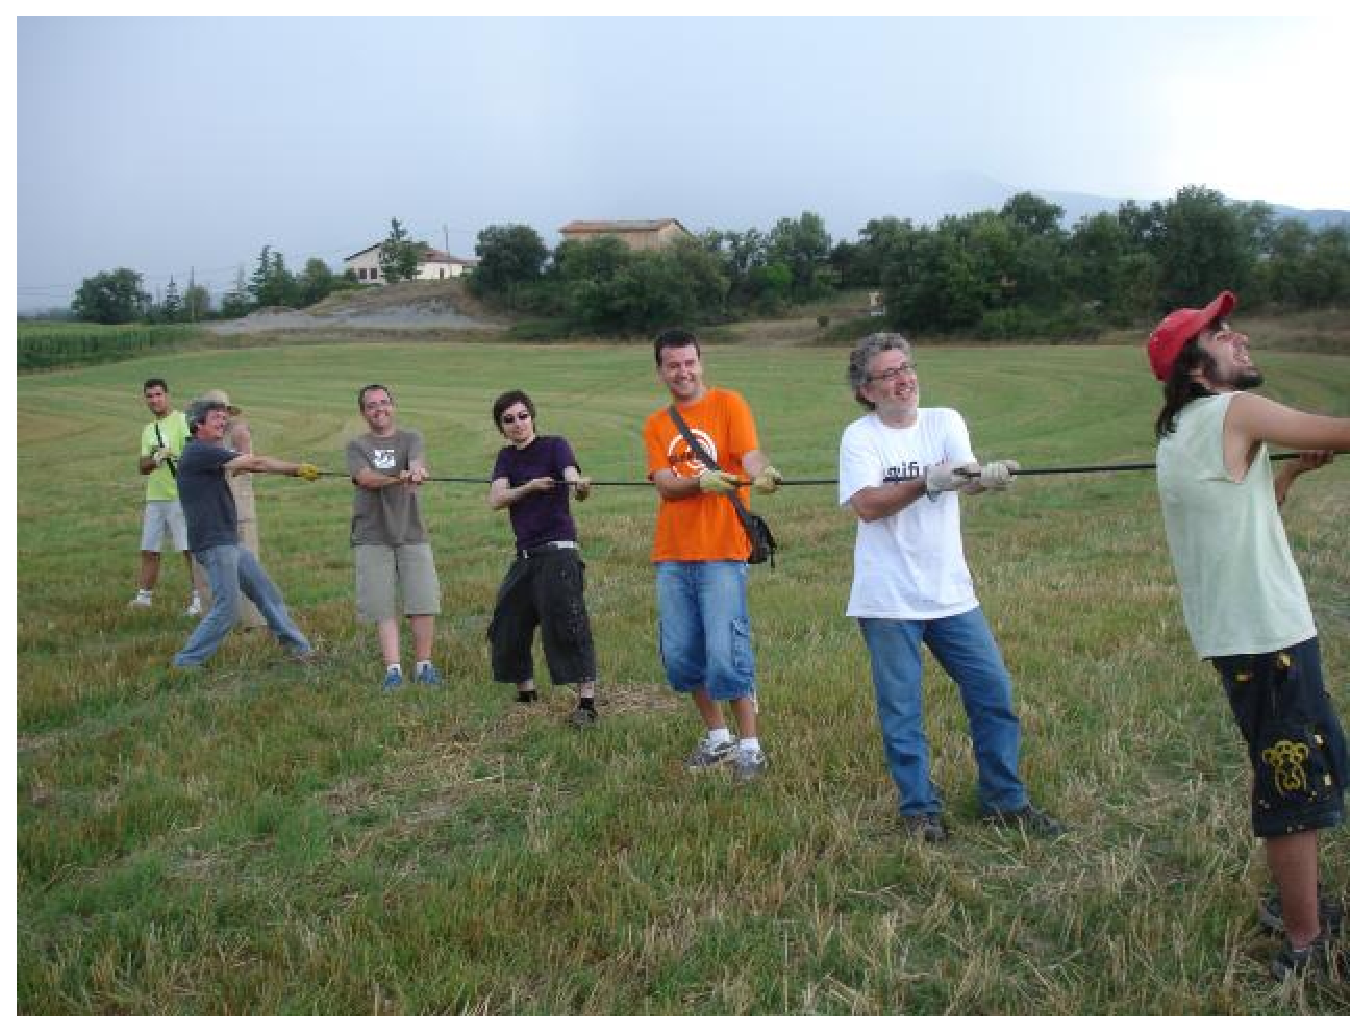
\includegraphics{sect2/figures/Gurb_it1_pic1.eps}} &
      \resizebox{70mm}{!}{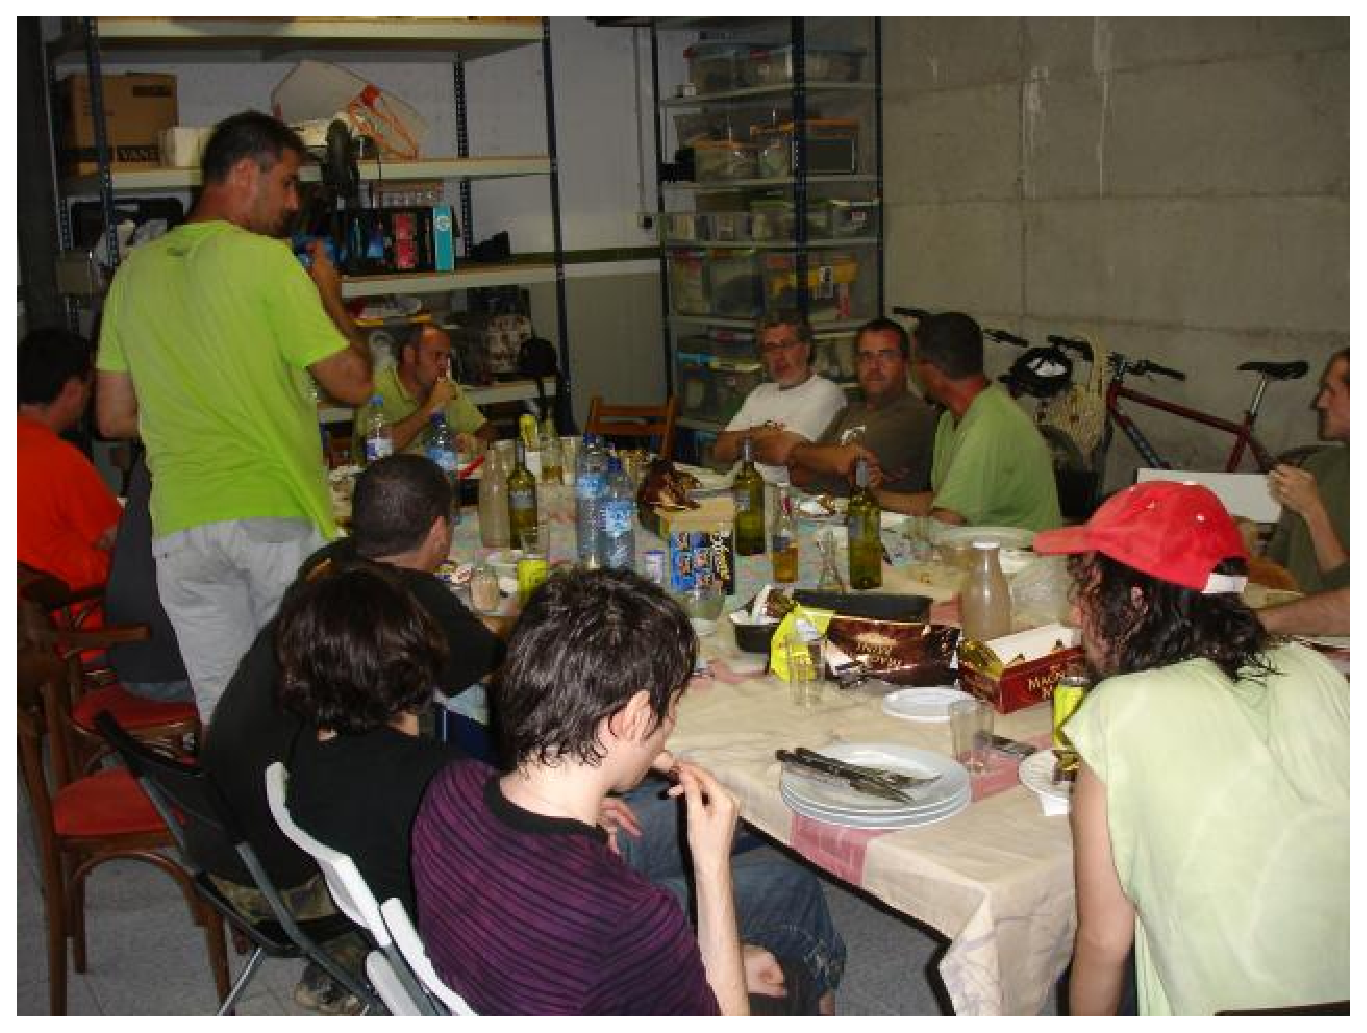
\includegraphics{sect2/figures/Gurb_it1_pic2.eps}} \\
      \resizebox{70mm}{!}{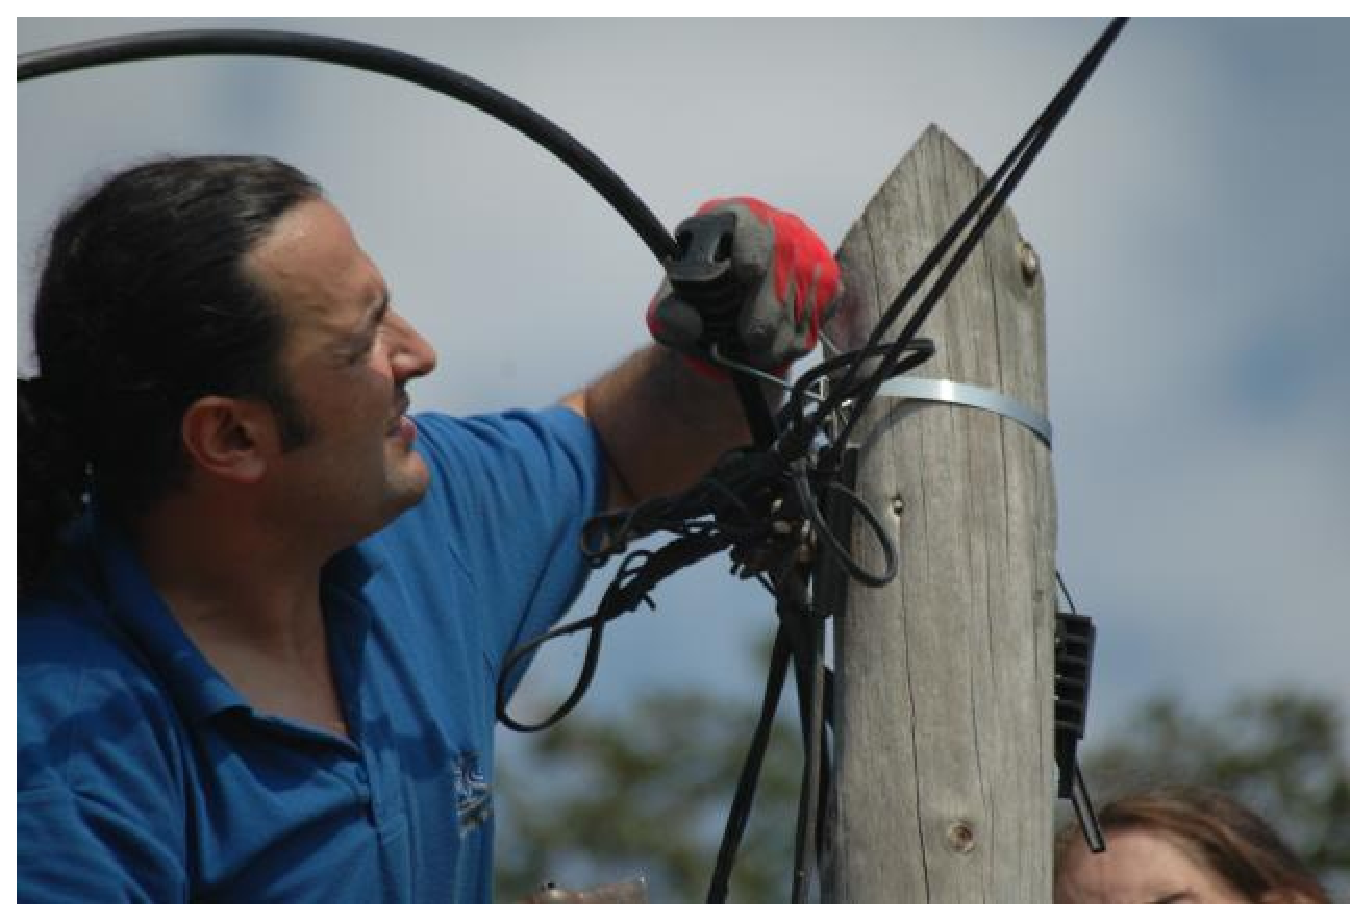
\includegraphics{sect2/figures/Gurb_it1_pic3.eps}} &
      \resizebox{70mm}{!}{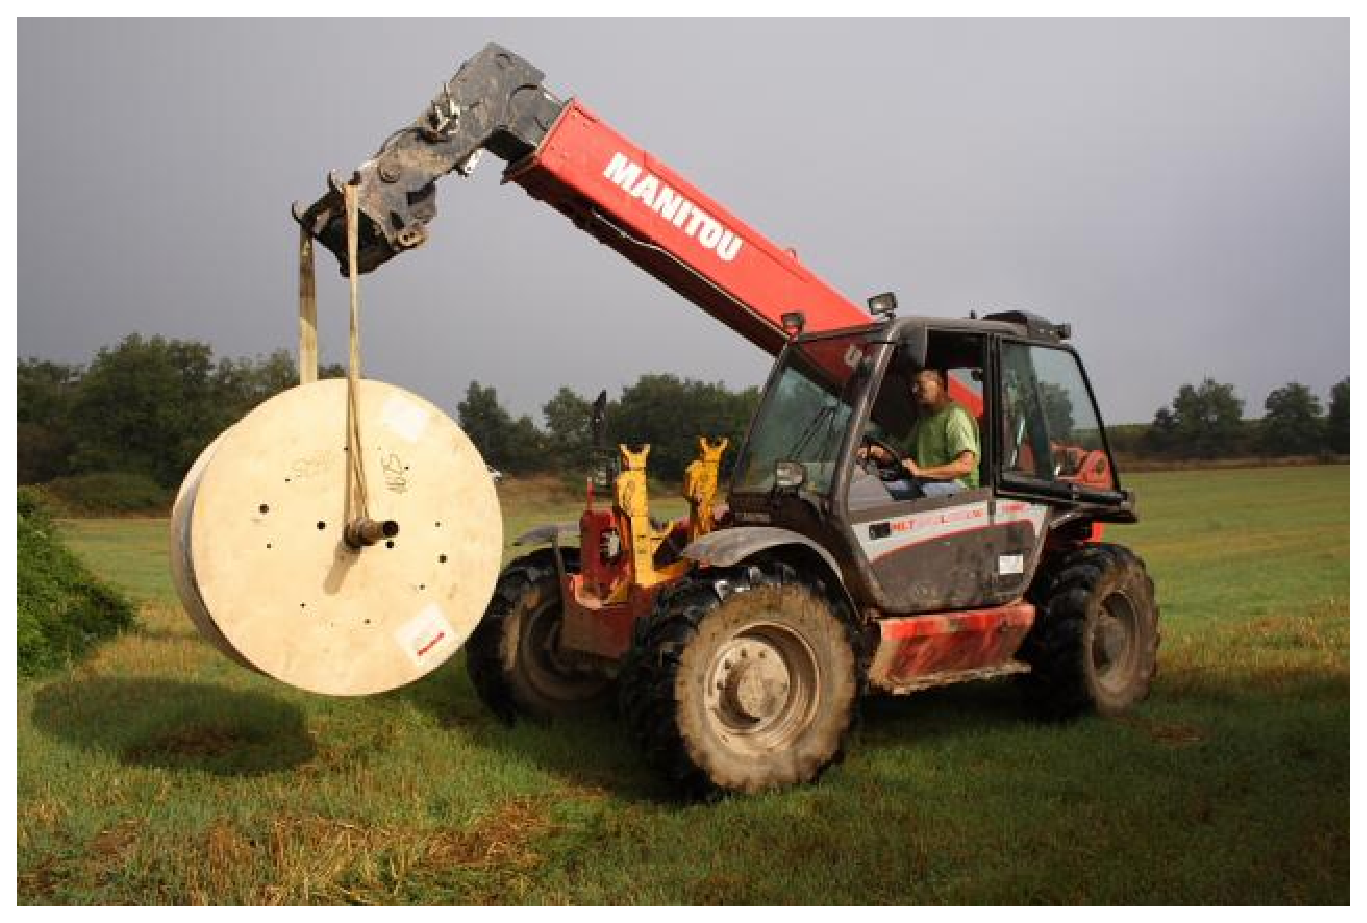
\includegraphics{sect2/figures/Gurb_it1_pic4.eps}} \\
    \end{tabular}
  \caption{OF deployment in Gurb's first iteration. Pictures of the deployment execution, August 2009.}
  \label{fig:gurb_it1_pics}
\end{figure}

\begin{figure}[htbp]
  \centering
  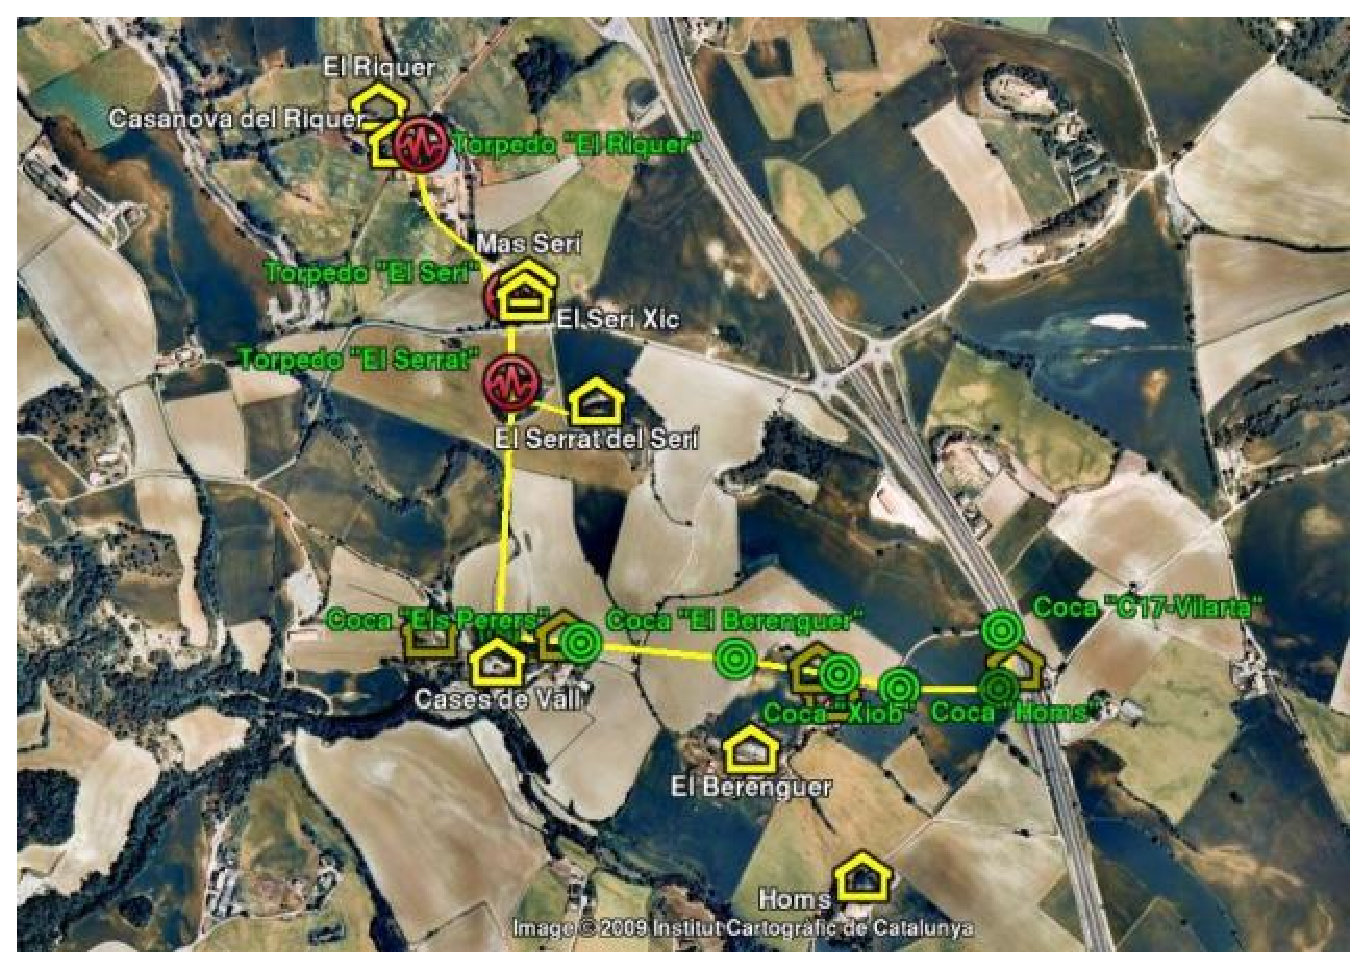
\includegraphics[scale=.65]{sect2/figures/Gurb_it1_map.eps} 
  \caption{OF deployment in Gurb's first iteration. Map. Executed in 2009.}
  \label{fig:gurb_it1_map}
\end{figure}

In 2012 the second iteration was started\footnote{\url{http://guifi.net/es/node/50325}}. It is expected to be finished at the very beginning of 2013. 

\begin{figure}[htbp]
  \centering
  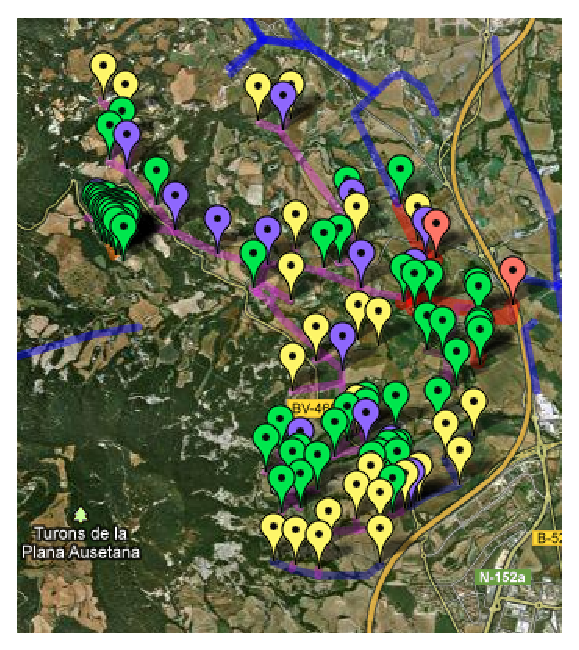
\includegraphics[scale=1.3]{sect2/figures/Gurb_it2_map.eps} 
  \caption{OF deployment in Gurb's fist iteration. Map. Blue spots are the \emph{Passive Optical Splitters}, green spots are homes connected as of the beginning of December 2012, yellow spots are homes to be connected by the end of this iteration.}
  \label{fig:gurb_it2_map}
\end{figure}

The third iteration is scheduled for 2013 and 2014. In this iteration urban areas will be wired. To do so local government ducts and dark fibers will be used.

Gurb deployments is the testbed where the Bottom-up Broadband (BuB) model has been tested. Due to its success it has become a reference for the guifi.net community.

\FloatBarrier
\subsubsection{Vic}

Vic\footnote{Vic, population 40.900 hab, density 1.336,60 hab/km$^{2}$, the capital of the ''comarca'' of Osona, Catalonia.} is a typical middle size Catalan city of the Catalan rural areas where most of the population lives in the urban area with several industrial parks. It is neighbouring Gurb. Initial guifi.net nodes were set up in 2003. The local government has gradually increased the commitment to the project up to the point to make available its ducts to deploy OF according to guifi.net's principals. At the moment the access to the local government dark fibers is being negotiated.

Initial attempts to deploy OF dates back to 2009. In 2011 the Catalan government proposed to the guifi.net Foundation to organise a summer camp\footnote{\url{http://blogs.guifi.net/camp2012/}} meant for teenagers. As a result of it the first iteration was executed in August 2012 and activated next month. Summer camp attendees actively participated in the whole process of OF deployment. Figure~\ref{fig:vic_it1_pics} shows some pictures of the summer camp. Figure~\ref{fig:vic_sc12} presents the map of this iteration. In this case non-residential buildings where connected. More precisely, a primary school\footnote{Escola Andersen, students from 3 to 11 years old, 600 students, \url{http://www.xtec.cat/ceipandersen/}.}, a students residence\footnote{Alberg de Joventut Canonge Collell, 100 rooms, Generalitat de Catalunya, \url{http://www10.gencat.cat/sac/AppJava/organisme_fitxa.jsp?codi=2549}.}, a sport resort\footnote{Club Patí Vic, 2000 members, first hockey Spanish league, \url{http://www.clubpativic.net/clubpativic/index.php/ca/}.} and a weather station. At the moment of the deployment the fastest Internet connection offered by the traditional telcos to these buildings was: primary school 0.5Mb/s, students residence 2Mb/s, sport resort 2Mb/s, weather station 1Mb/s.

\begin{figure}[htbp]
  \centering
    \begin{tabular}{cc}
      \resizebox{70mm}{!}{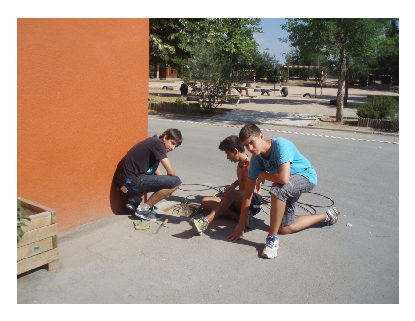
\includegraphics{sect2/figures/Vic_it1_pic1.eps}} &
      \resizebox{70mm}{!}{
\includegraphics{sect2/figures/Vic_it1_pic2.eps}} \\
      \resizebox{70mm}{!}{
\includegraphics{sect2/figures/Vic_it1_pic3.eps}} &
      \resizebox{70mm}{!}{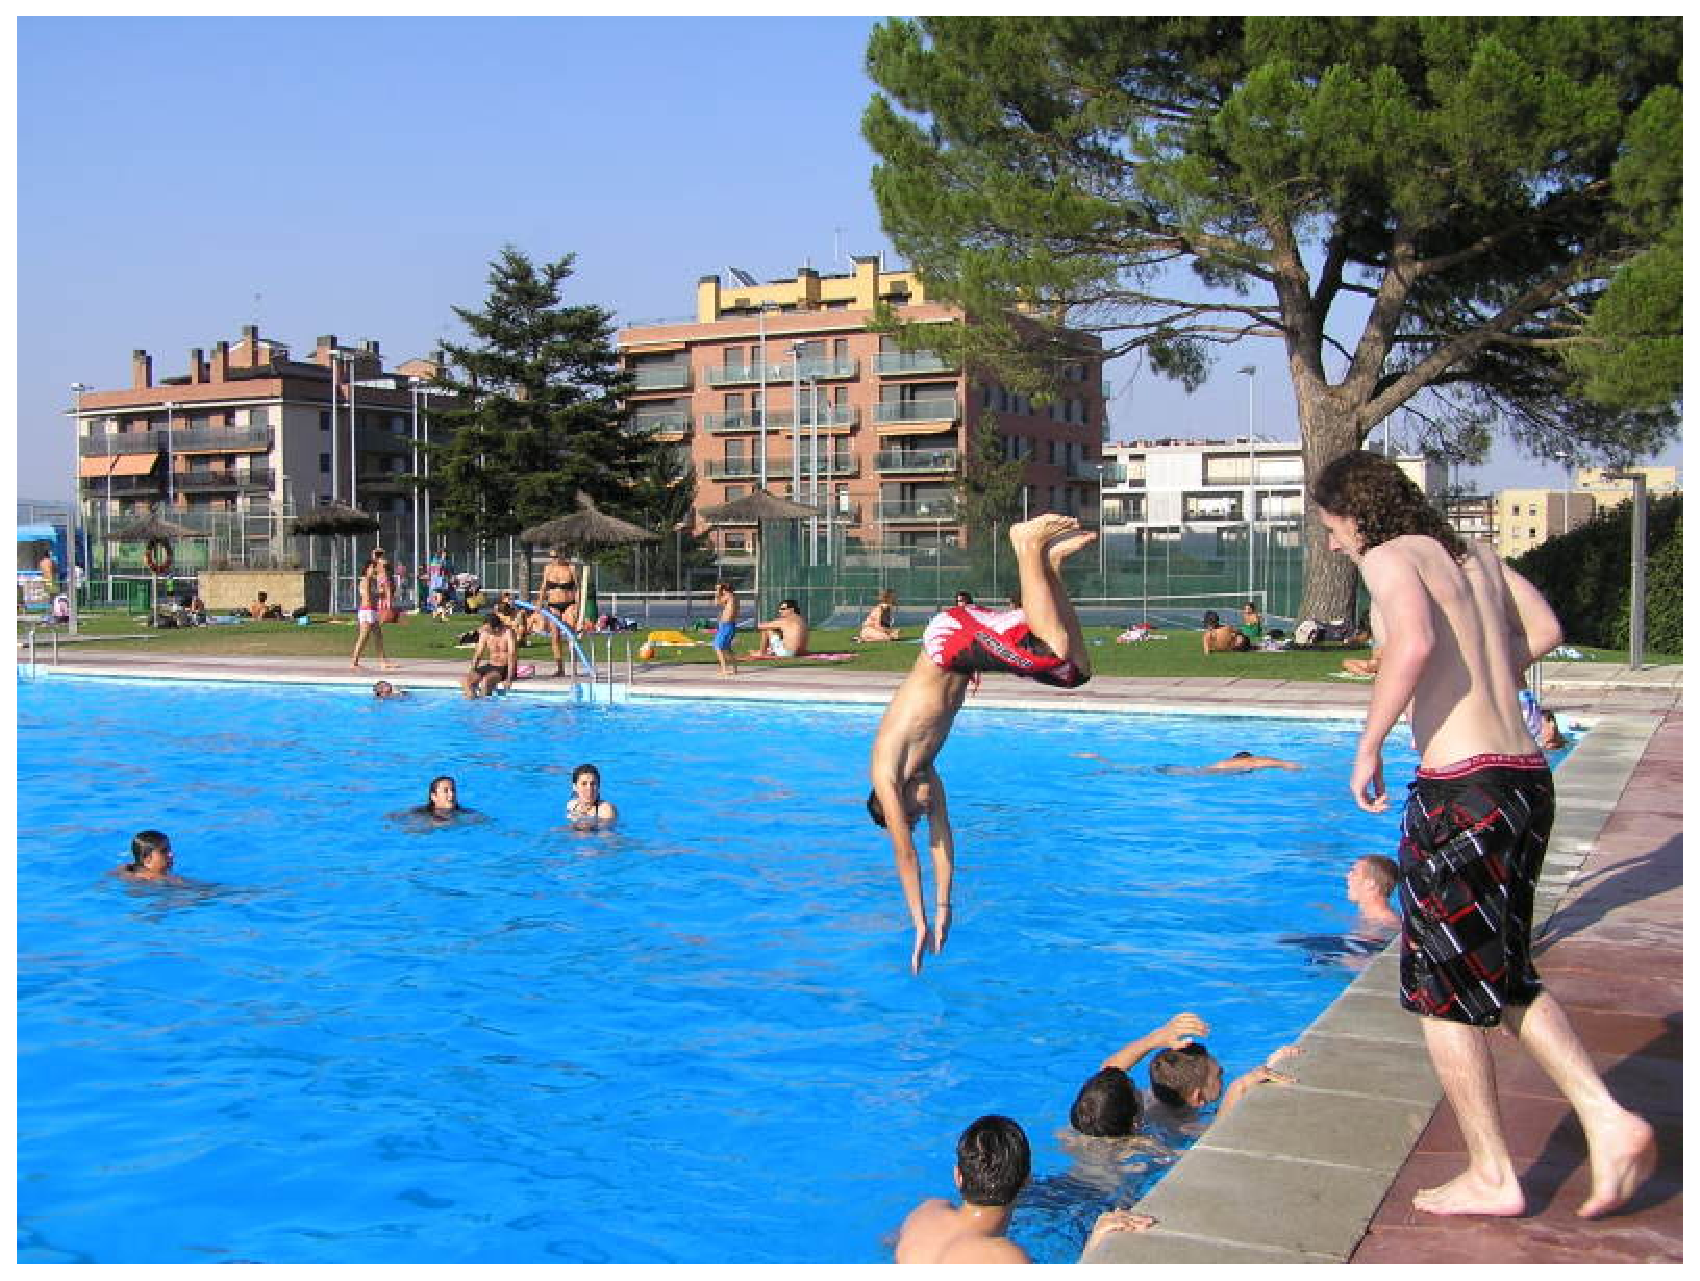
\includegraphics{sect2/figures/Vic_it1_pic4.eps}} \\
    \end{tabular}
  \caption{OF deployment in Vic's first iteration. Pictures of the deployment execution during the summer camps August 2012.}
  \label{fig:vic_it1_pics}
\end{figure}


\begin{figure}[htbp]
  \centering
  \includegraphics[scale=.33]{sect2/figures/Vic_summer_camp_2012.eps} 
  \caption{OF deployment in Vic's first iteration. Executed in 2012. Result of a teenager's summer camp.}
  \label{fig:vic_sc12}
\end{figure}

Currently the second iteration is already started and it is expected to be finished by 2013. Figure~\ref{fig:vic_it1} presents the map of this iteration.

\begin{figure}[htbp]
  \centering
  \includegraphics[scale=.33]{sect2/figures/Vic_iteration1.eps} 
  \caption{OF deployment in Vic second iteration. Planned for 2013.}
  \label{fig:vic_it1}
\end{figure}





\FloatBarrier
\subsubsection{Rub\'{i}}

Rub\'{i}\footnote{Rub\'{i}, population 73.979 hab, density 2.290,37 hab/km$^{2}$, located in the ''comarca'' of Vall\`{e}s Occidental, Catalonia.} is a typical middle size Catalan city of the Barcelona surroundings where most of the population lives in the urban with several industrial parks.

Rub\'{i} local government in early 2012 showed interest in deploying fiber following a Bottom-up Broadband model.
The first goal was to offer high-speed Internet connections to the largest companies operating in one of Rub\'{i}'s industrial areas called ''Can Jardi''.
These companies had access only to slow ADSL connections and the absence of a fiber deployment was seriously affecting their competitiveness.
The lack of commercial high speed connections offering prompted the city's local government to look for alternatives.

An initial round of conversations took place in Spring 2012 to plan for a deployment during the Summer.
The planning involved a strong participation of a local partner, company with experience in wireless BuB deployment.
This initial planning for a bottom-up-broadband deployment did not pass unnoticed, and commercial ISPs approached the Rub\'{i} local government with fiber deployment offerings.
The offering was to place the city of Rub\'{i} high in de ISPs fiber deployment plans and prioritize it over other cities.
Guifi, UPF and the local partner were asked by the city's local government to prepare a concrete offering that could match the offering of the ISPs.

The arrival of traditional ISPs proposals, combined with the uncertainties of the competence of the local partner to carry out fiber deployments and internal discrepancies in the Rub\'{i}'s local government slowed down the pilot.
Currently this pilot is on hold, and it is not clear how it will resolve.
Personal interests and personal connections within the City Hall may play an important role in the final resolution.

It is remarkable that the fact that the City Hall entered in conversations to plan a BuB deployment triggered a number of events that placed the city in a much favourable situation to negotiate with the ISPs about future fiber deployments.


\FloatBarrier
\subsection{Other deployments}

Aside from the deployments already presented there are other OF initiatives in guifi.net. Table~\ref{tab:other_deployments} summarises them.

\begin{table}[htbp]
  \centering
    \begin{tabular}{|p{2cm}|p{4cm}|p{8cm}|}
      \hline \textbf{Project} & \textbf{Status} & \textbf{Comments} \\ \hline \hline
      Taradell & First iteration executed & Interconnection of a secondary school with guifi.net local POP \\ \hline
    \end{tabular}
  \caption{Other deployments.}
  \label{tab:other_deployments}
\end{table}